\documentclass[../main.tex]{subfiles}
\graphicspath{{\subfix{../images/}}}

\begin{document}


\subsection{Decision Tree}

\subsubsection{Hyper Parameters}

To reduce the computational cost of training the classifier, we 
used a subset of the the extracted features from the principle 
components analysis. We determined our features to be the first 
$62$ principal components. We saw earlier that the first $62$ 
principal components had a cumulative explained variance ratio of $90\%$. 
We found that a CVR of $90\%$ was sufficient since it reduced the feature 
dimensionality and thereby the cost of training while also 
preserving most of the information from the original data set.
This data set of $62$ standardised principal components from 
the training set was then used to find the best hyper parameters 
for our model. 
The different hyper parameters our model provides limits to 
(splitting) \inlinecode{criterion}, \inlinecode{max_depth} and 
\inlinecode{min_samples_leaf}. 
Given that we only have three hyper parameters, we found it 
suitable to perform a grid search to find the hyper parameters 
that yield the best performing classifier. 
For the grid search, we chose \inlinecode{max_depth} with a range 
from $1$ to $20$, and \inlinecode{min_samples_leaf} with a range 
from $1$ to $30$ and the splitting criterion to be either Gini or 
Entropy.

The \inlinecode{GridSearchCV} from scikit-learn considers all 
possible combinations of the parameters. For each combination it 
fits the model and computes the mean accuracy, using k-fold cross 
validation with $k$ set to $5$. We are then able to call 
\inlinecode{best_params_} in order to obtain the combination of 
the given hyper parameters that results in the best accuracy 
score out of the given options. 
The hyper parameters that resulted in the best performance on the 
validation splits were a max depth of $15$, minimum number of 
samples in a leaf node $21$ and Gini Impurity as the splitting 
criterion. 


\subsubsection{Results and Performance}

The fitted and trained decision tree, with the best performing 
hyper parameters, resulted in an accuracy score of $76\%$ on the 
test split. As depicted in 
(\autoref{tab:dt_test_scores}) the classifier is  insufficient at 
predicting class $4$ (Shirt), looking at the F1-score, but 
adequate at predicting the other classes. 

\begin{table}[H]
    \centering
    \vspace{2em}
\rowcolors{2}{white}{custom_grey}
\begin{tabular}{lllllll}
&  \hspace{0.2em}\begin{rotate}{45} T-shirt/top \end{rotate}  &  \hspace{0.2em}\begin{rotate}{45} Trouser \end{rotate}  &  \hspace{0.2em}\begin{rotate}{45} Pullover \end{rotate}  &  \hspace{0.2em}\begin{rotate}{45} Dress \end{rotate}  &  \hspace{0.2em}\begin{rotate}{45} Shirt \end{rotate} \\
 \toprule
 Precision                       &                  0.73                  &                   0.96                    &                   0.75                   &                   0.80                   &                   0.57\\
 Recall                          &                  0.72                  &                   0.91                    &                   0.77                   &                   0.82                   &                   0.57\\
 F1-score &                  0.73                 &                   0.93                    &                   0.76                   &                   0.81                   &                   0.57\\
 \midrule
Training Accuracy & & & & & & 0.90\\
Test Accuracy & & & & & & 0.76\\

 \bottomrule
\end{tabular}
    \caption{Decision tree results}
    \label{tab:dt_test_scores}
\end{table}

A decision tree is a model with high variance. This means that a 
small change in the data can result in a major change in the 
structure of the tree and ultimately convey a different result. 
We make our prediction based on one decision tree only, and 
therefore expect the classifier to have high variance. This might 
explain the considerable drop in accuracy when evaluating the 
model on the test set. Often one would use bagging or boosting to 
prevent this. 

Using principle component analysis for dimensionality reduction 
is a very useful technique, considering the fact that it can 
prevent overfitting, improve performance and make computations 
less expensive. Nevertheless, principle components are 
troublesome to interpret. Even though a decision tree classifier 
is an easyly interpretable model, it is difficult to illustrate 
which features are more important than others when we use 
principle components. Additionally, to some extent, a part of the 
information is lost when dimensions are reduced. Choosing the 
number of principal components is a trade-off between 
dimensionality and information loss. Choosing a small number of 
principal components amounts in a substantial dimensionality 
reduction, and thus reducing computation. However, it also 
increases information loss.


\subsection{Neural Network}

\subsubsection{Hyper Parameters and Architecture}

The selection of hyper parameters in our feed-forward neural 
network implementation was boundless, considering the fact that 
the structure of the model can be so vast. Therefore systematic 
optimisation strategies for a complex model like this, can be 
very exhaustive and computationally expensive. Hence the model 
selection in this case, was based on trial and error. 


The final structure of our feed-forward neural network consisted 
of three layers with a single hidden layer. The first (input) 
layer with $32$ neurons. The hidden layer consisted of $16$ 
neurons, and the last (output) layer consisted of $5$ neurons. 
Both the input layer and the hidden layer had Leaky ReLU 
activation functions, and the output layer had a softmax 
activation function.
We standardised the input with the scikit-learn 
\inlinecode{StandardScaler} instance before feeding it to the 
network. We ran $75$ epochs with the training data split into 
$100$ batches and a learning rate of $0.0001$.


\subsubsection{Results and Performance}

The fitted and trained Neural Network performed with a training 
accuracy of $99\%$ and a test accuracy of $85\%$.
Looking at \autoref{tab:ffnn_test_scores}, it is clear to see 
from the F1-score that the model is great at predicting class $1$ 
(Trousers), but less precise at class $4$ (Shirts). 

\begin{table}[H]
    \centering
    \vspace{2em}
\rowcolors{2}{white}{custom_grey}
\begin{tabular}{lllllll}
&  \hspace{0.2em}\begin{rotate}{45} T-shirt/top \end{rotate}  &  \hspace{0.2em}\begin{rotate}{45} Trouser \end{rotate}  &  \hspace{0.2em}\begin{rotate}{45} Pullover \end{rotate}  &  \hspace{0.2em}\begin{rotate}{45} Dress \end{rotate}  &  \hspace{0.2em}\begin{rotate}{45} Shirt \end{rotate} \\
 \toprule
 Precision                       &                  0.80                  &                   0.97                    &                   0.83                   &                   0.90                   &                   0.72\\
 Recall                          &                  0.81                  &                   0.96                    &                   0.87                   &                   0.88                   &                   0.70\\
F1-score &                  0.80                  &                   0.97                    &                   0.85                   &                   0.89                   &                   0.71\\
 \midrule
Training Accuracy & & & & & & 0.99\\
Test Accuracy & & & & & & 0.84\\

 \bottomrule
\end{tabular}
    \caption{Feed-forward neural network results}
    \label{tab:ffnn_test_scores}
\end{table}
 
A problem we encountered with our neural network implementation 
was overfitting. This is not surprising since all standard, fully 
connected neural network architectures are prone to overfitting 
\autocite{prechelt_early_2012}. Our implementation does not have 
any methods that prevent overfitting, since we chose to keep the 
model simple. Normally you could prevent this by implementing 
early stopping. That is we break the training when a parameter 
update no longer improves the validation data. This is a common 
regularisation technique for deep learning models, to avoid poor 
performance. Overfitting can also be prevented by using other 
regularisation methods like drop-out, L1 and L2 regularisation. 


\subsection{Convolutional Neural Network}

\subsubsection{Introduction}

We have chosen our third model to be a convolutional neural 
network.
When working with normal feed-forward neural networks you lose the 
structure of the image, since you need to flatten the image array.
This is where convolutional neural networks really shine, since 
the structure of the image is preserved.
To some degree they mimic how we, as humans classify images which 
is by recognising specific patterns and features anywhere in the 
image that differentiate each distinct object class.

The architechture of a convolutional neural network consists of 
two major parts, a feature learning/extraction part and a 
classification part. The classification part, is constructed in 
the same way as a normal feed-forward neural network.


\subsubsection{Convolutional and Pooling Layers}

A convolutional layer is made up of a number of convolutional 
filters or kernels, each of these are templates that help 
determine whether a particular local feature is present in an 
image or not. These features are then combined to form higher-level features, such as parts of eyes, ears and the like.
A kernel relies on a simple operation, called a 
\textit{convolution}, which essentially amounts to repeatedly 
multiplying matrix elements and summing the results 
\autocite{JamesStatisticalLearning}. 
A \textit{pooling} layer provides a way to condense a large image 
into a smaller summary image. There are numerous ways to perform 
pooling.

Both the convolutional layers and the pooling layers help reduce 
the spacial size of the convolved feature. This is done to 
decrease the overall computational power required to process the 
data via dimensionality reduction. In the end the presence or 
absence of these high-level features help determine the 
probability of any given output class.


\subsubsection{Hyper Parameters and Architecture}

For the convolutional neural network we used the LeNet-5 
architecture (\autoref{fig:LeNet-architechture}). 

\begin{figure}[ht]
    \centering
    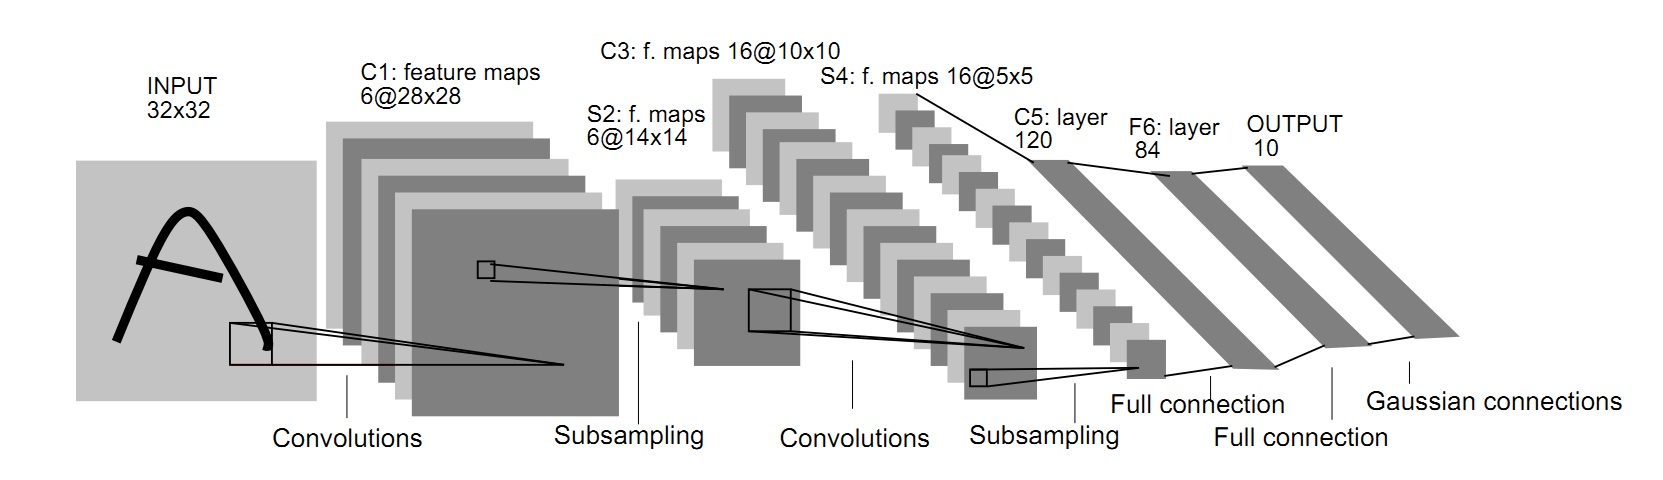
\includegraphics[width=\textwidth]{lenet-5}
    \caption{LeNet-5 convolutional neural network architecture}
    \label{fig:LeNet-architechture}
\end{figure}

This architecture was proposed by Yann LeCun and others in 1998 
for recognising handwritten and machine-printed characters 
\autocite{lecun-lenet}. Since then LeCun has been recognised as a 
founding father of convolutional neural networks.

Because the LeNet-5 architecture was created for recognising 
characters in different data sets, including the MNIST data set 
\autocite{digit_mnist}, we figured that the same architecture 
would be well suited for the Fashion MNIST data set as well. 
Compared to our own feed-forward neural network we were able to 
implement early stopping, to prevent overfitting. 


\subsubsection{Results and Performance}

The fitted LeNet-5 convolutional neural network performed with a 
training accuracy of $92\%$ and a test accuracy of $87\%$. As we 
expected the model is better at correctly distinguishing and 
predicting the classes, that our own neural network struggled 
with (\autoref{tab:cnn_test_scores}).

\begin{table}[ht]
    \centering
    \vspace{2em}
\rowcolors{2}{white}{custom_grey}
\begin{tabular}{lllllll}
 &  \hspace{0.2em}\begin{rotate}{45} T-shirt/top \end{rotate}  &  \hspace{0.2em}\begin{rotate}{45} Trouser \end{rotate}  &  \hspace{0.2em}\begin{rotate}{45} Pullover \end{rotate}  &  \hspace{0.2em}\begin{rotate}{45} Dress \end{rotate}  &  \hspace{0.2em}\begin{rotate}{45} Shirt \end{rotate} \\
 \toprule
 Precision                       &                  0.80                  &                   0.98                    &                   0.88                   &                   0.95                   &                   0.75\\
 Recall                          &                  0.87                  &                   0.97                    &                   0.89                   &                   0.88                   &                   0.73\\
F1-score &                  0.83                 &                   0.98                    &                   0.88                   &                   0.91                   &                   0.74\\
 \midrule
Training Accuracy & & & & & & 0.92\\
Test Accuracy & & & & & & 0.87\\

 \bottomrule
\end{tabular}
    \caption{LeNet-5 convolutional neural network results}
    \label{tab:cnn_test_scores}
\end{table}


\end{document} 